\vfill\null\columnbreak
\section{Reglerauslegung}
    \subsection{PID-Regler}
        \begin{center}
           \begin{tabular}{|c|c|c|}
              \textbf{Proportionalregler}  & (\textbf{P}-Term) & $e(t)$ \\
               \textbf{Integralregler} & (\textbf{I}-Term) & $\frac{1}{T_i}\cdot\int_0^t e(\tau)d\tau$ \\
               \textbf{Derivative-Term} & (\textbf{D}-Term) & $T_d\cdot\frac{d}{dt}e(t)$
           \end{tabular}
        \end{center}
        Der \textbf{I}-Term wird betragsmässig grösser, je länger ein einseitger Fehler (z:B. $e(t) > 0$) vorhanden ist. 
        Der \textbf{D}-Term wirkt auf schnelle Änderungen im Fehlersignal. Ein Nachteil des D-Terms ist, dass er Rauschen auf dem Fehlersignal $e(t)$ verstärkt.
          
        Eine Transformation in den Frequenzbereich ergibt
        \begin{center}
        \begin{tabular}{|c|c|c|}
          \textbf{Proportionalregler}  & (\textbf{P}-Term) & $1$ \\
           \textbf{Integralregler} & (\textbf{I}-Term) & $\frac{1}{T_i\cdot s} $\\
           \textbf{Derivative-Term} & (\textbf{D}-Term) & $T_d\cdot s$
        \end{tabular}
        \end{center}
        
        Im Zeitbereich sieht ein PID-Regler folgendermassen aus.
        
       \[U_\textrm{PID}(t) = k_p\cdot\Bigg(e(t)+ \frac{1}{T_i}\cdot\int_0^t e(\tau)d\tau +T_d\cdot\frac{d}{dt}e(t)\Bigg)\]
       
       in den Frequenzbereich transformiert ergibt sich folgendes:
       \[C_\textrm{PID}(s) = k_p\cdot\Bigg(1+\frac{1}{T_i\cdot s} + T_d\cdot s\Bigg)=\frac{U(s)}{E(s)}
       \]
       Da der D-Term sehr empfindlich auf Rauschen ist werden hohe Frequenzen ganz einfach unterdrückt, indem man eine hochfrequente doppelte Nullstelle an den Regler hängt. Sogenannte \textbf{roll-off} Term $\rightarrow \frac{1}{(\tau\cdot s+1)^2}$.
       \[C_\textrm{PID}(s) = k_p \cdot\overbrace{\Bigg(\underbrace{\frac{T_d\cdot T_i\cdot s^2+T_i\cdot s+1}{T_i\cdot s}}_\textrm{nicht kausal}\Bigg)\cdot  \frac{1}{(\tau\cdot s+1)^2}}^\textrm{kausal}\]
       
       Ohne den roll-off Term wäre die Übertragungsfunktion $\frac{U(s)}{E(s)}$ nicht kausal und entsprechen nicht praktisch realisierbar. Um $u(t)$ ohne roll-off zu berechnen, bräuchte man Zukunftswerte des Fehlersignals $e(t)$.\\\\
        \textbf{PID-Regler als Standardform im Frequenzbereich}
        \begin{center}
            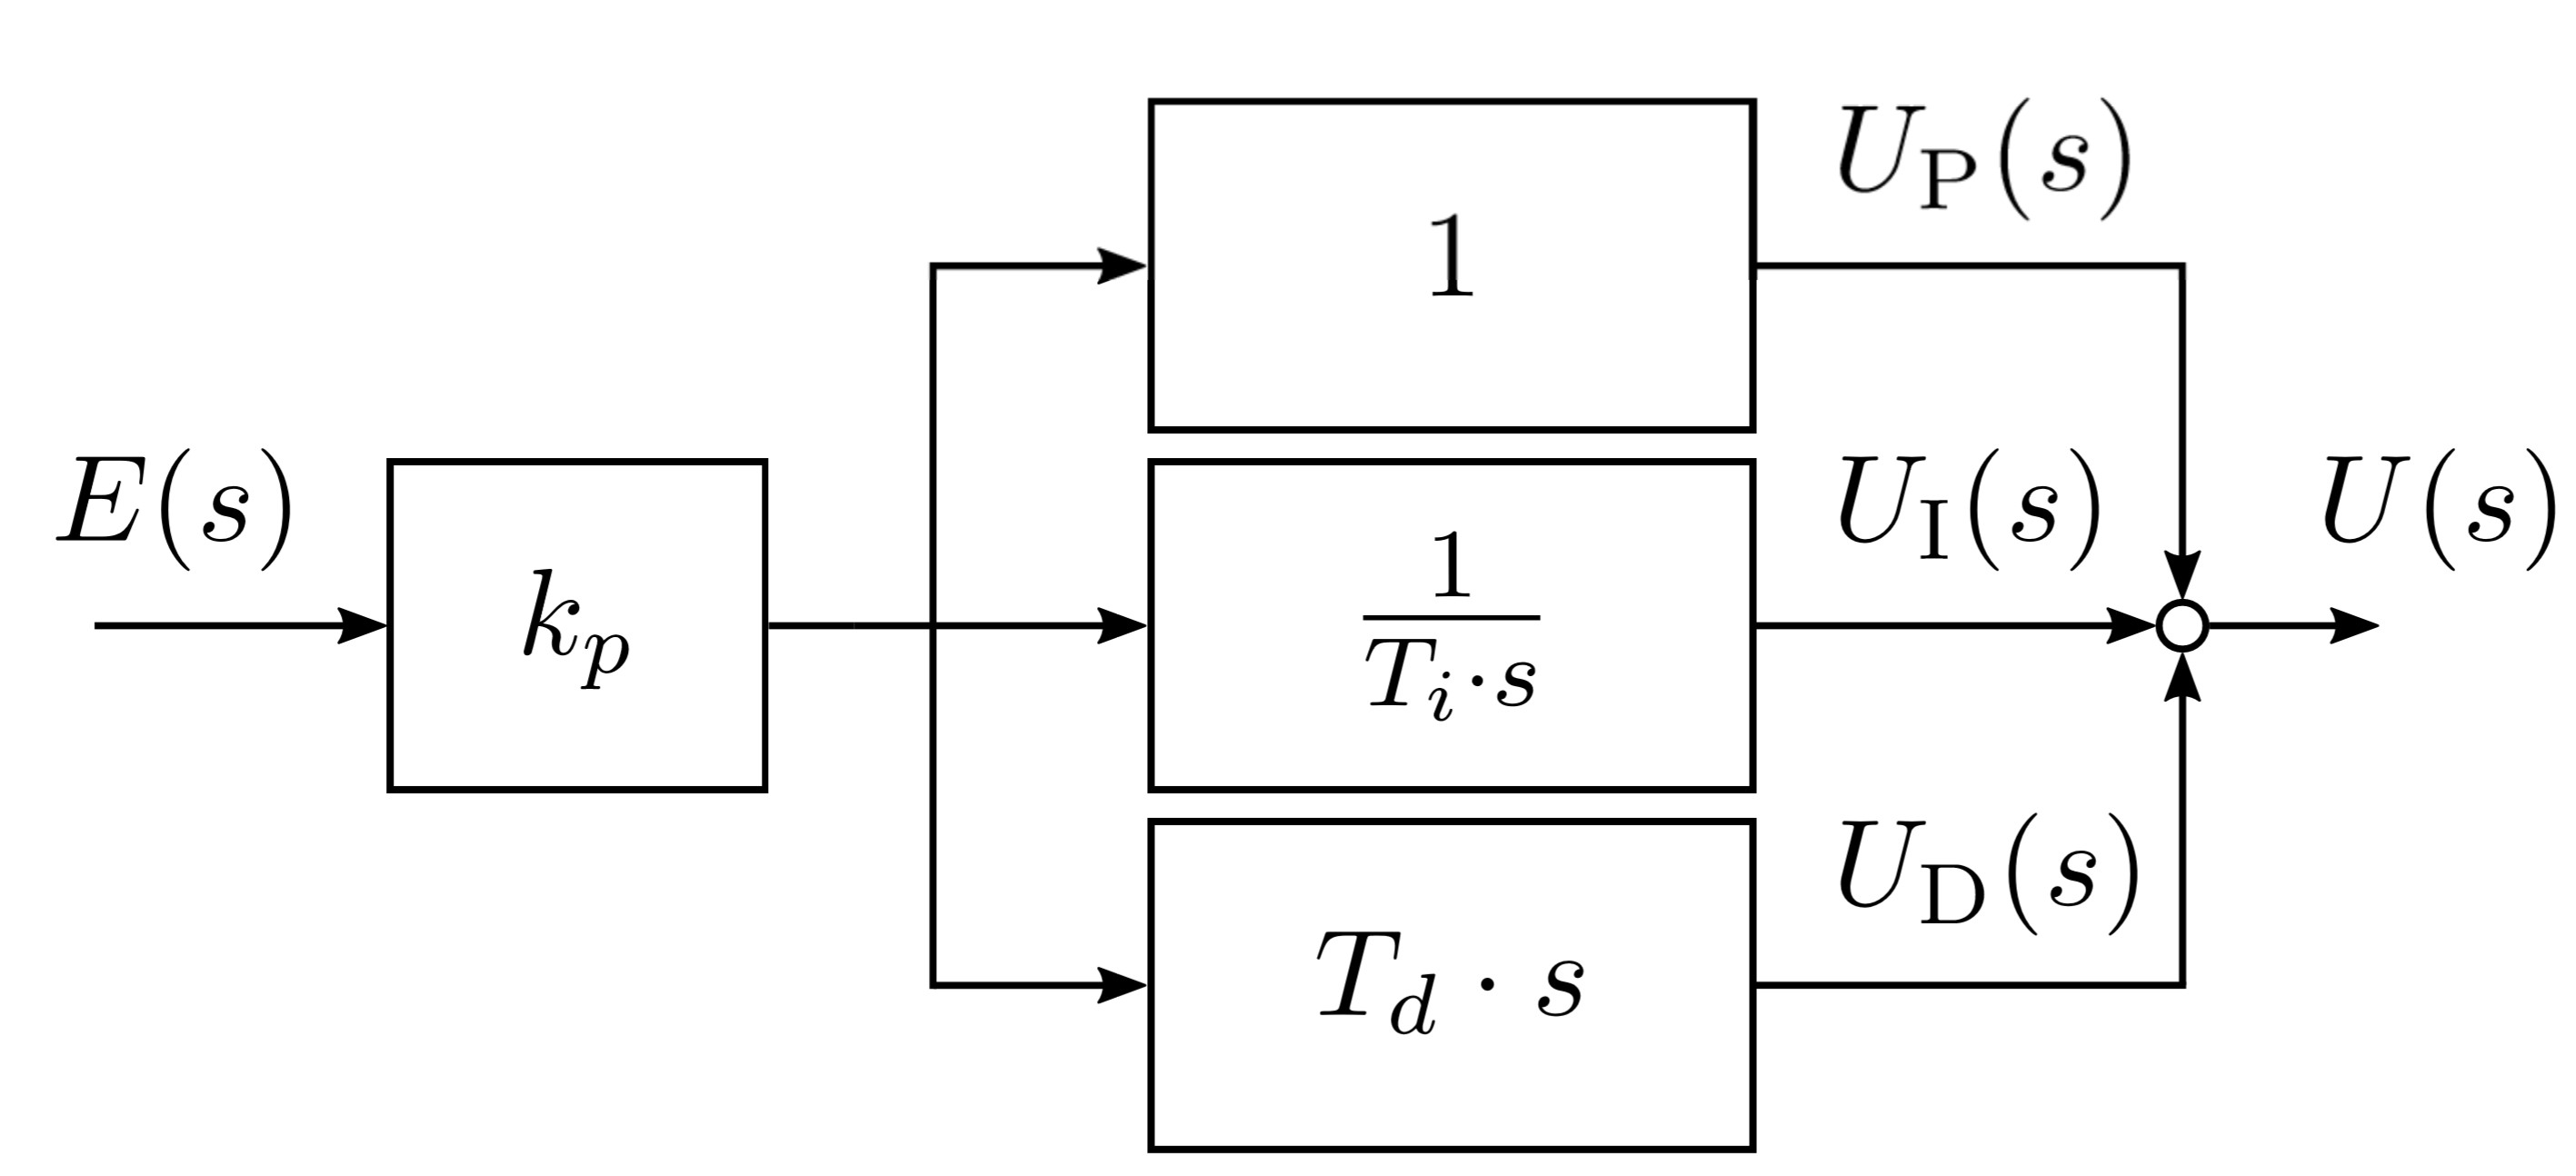
\includegraphics[width = 0.6\linewidth]{images/09/PID-regler.jpg}
        \end{center}
        
        \textbf{Pro Term ein Freiheitsgrad:} Dh. mit einem P Regler kann nur die Durchtrittsfrequenz \textit{ODER} die Phasenreserve eines Systems individuell verändert werden. Um beide Terme beinflussen zu können braucht man mehr Freiheitsgrade!
        
    \subsubsection{P-Term}
        \[
        u_\textrm{P}(t)= k_p\cdot e(t), \hspace{3mm} U_\textrm{P}(s) = k_p\cdot E(s)
        \]
        Der P-Term reagiert auf momentanen Wert des Fehlers $e(t)$. Die Stärke der Reaktion ist proportional zur Grösse des momentanen Fehlers.
    \subsubsection{I-Term}
        \[
        u_\textrm{I}(t) = \frac{k_p}{T_i}\cdot\int_0^te(\tau)d\tau, \hspace{3mm} U_\textrm{I}(s)=\frac{k_p}{T_i}\cdot\frac{1}{s}\cdot E(s)
        \]
        
        Der I-Term reagiert zum Zeitpunkt $t$ proportional auf den kumulierten Fehler, für $t\in[0,t]$. Falls ein statischer Nachlauffehler vorhanden ist, wird dieser aufintegriert, und der Reglerausgang wird immer grösser, bis kein Fehler mehr vorhanden ist. Ein Nachteil des Integrators ist, dass der Reglerausgang theoretisch beliebig gross werden kann.
        
        I-Terme führen immer zu einem \textbf{Phasenverlust}.
        
        \subsubsection{D-Term}
        \[u_\textrm{D}(t) = k_p\cdot T_d \cdot \frac{d}{dt}e(t),\hspace{3mm} U_\textrm{D}(s) = k_p\cdot T_d\cdot s\cdot E(s)\]
        
        Der D-Term wirkt antizipierend, er reagiert zum Zeitpunkt $t$ auf die momentane Änderungsrate des Fehlers. Der D-Term wirkt wie ein Dämpfer gegen ein schnelles Erhöhen oder Verringern des Fehlers. Eine starke Änderung im Fehler resultiert in einem erhöhten Reglerausgang. Falls die Änderung zu stark ist, kann der gewünschte Reglerausgang grösser als der grösst mögliche Eingang eines Systems werden. 
        
        D-Terme führen immer zu einem \textbf{Phasenanstieg}.
        \subsubsection{Bodediagramm eines PID-Reglers mit roll-off}
            \begin{center}
                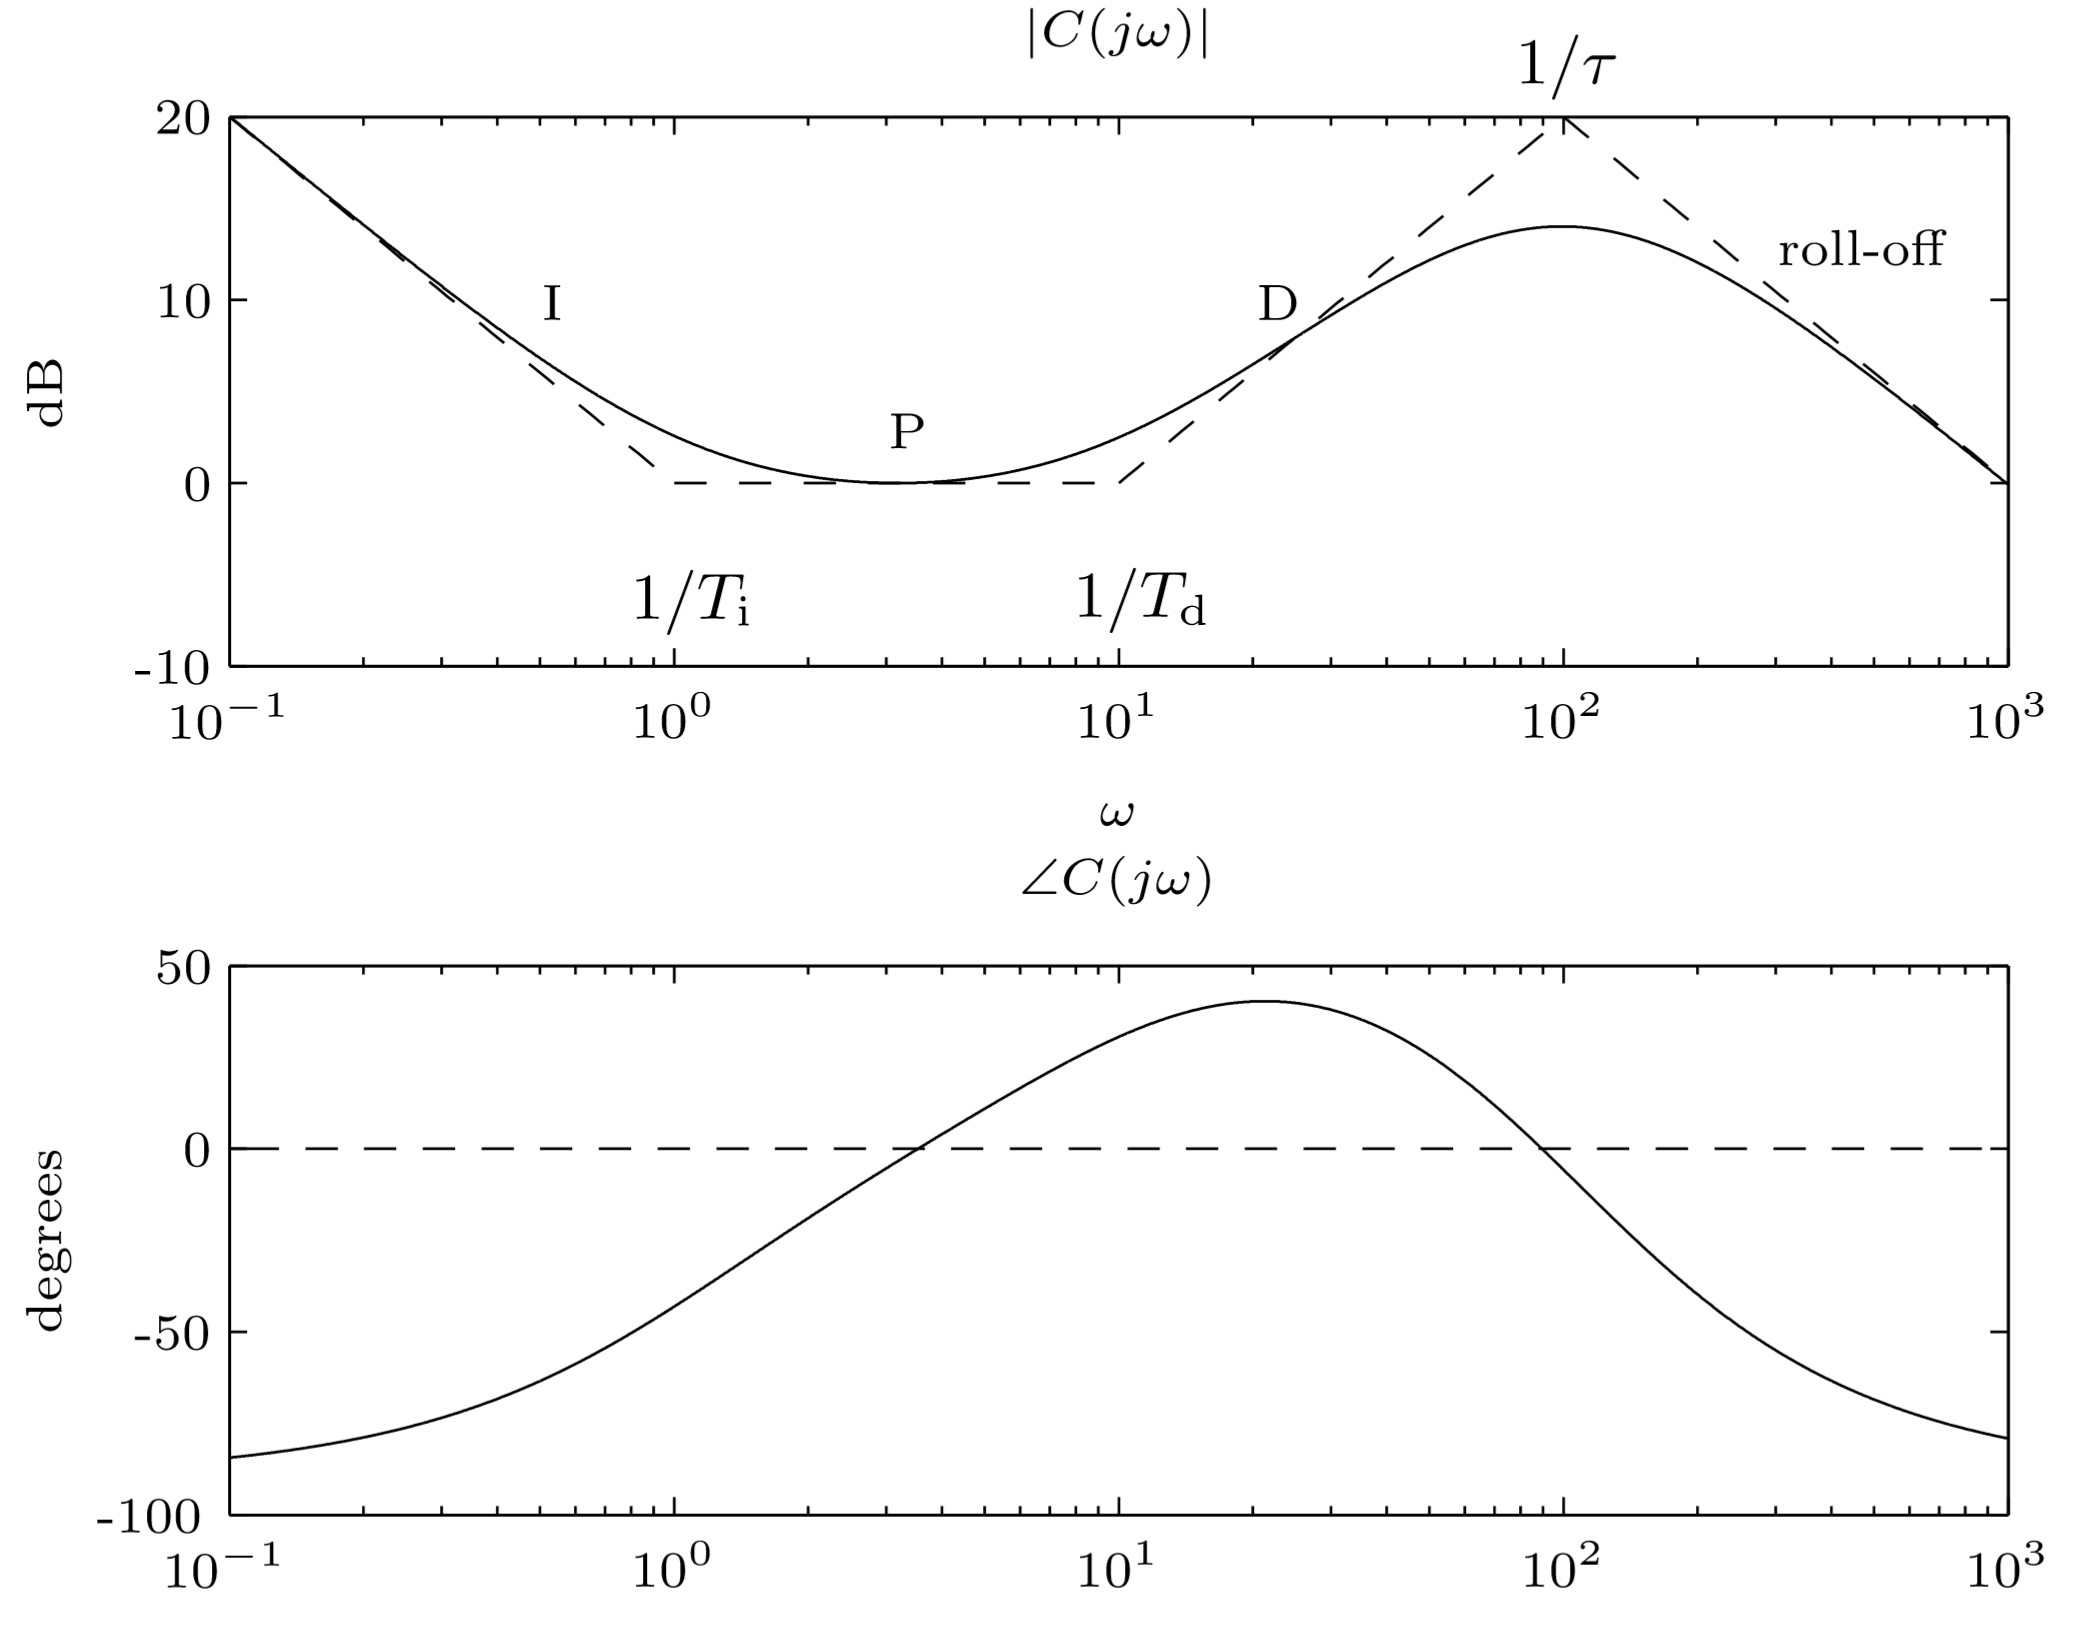
\includegraphics[width=\linewidth]{images/09/Bodediagramm_roll-off.jpg}
            \end{center}
        
        \subsubsection{Bsp}
            \textbf{Regelung eines Systems 2. Ordnung}
            \begin{center}
                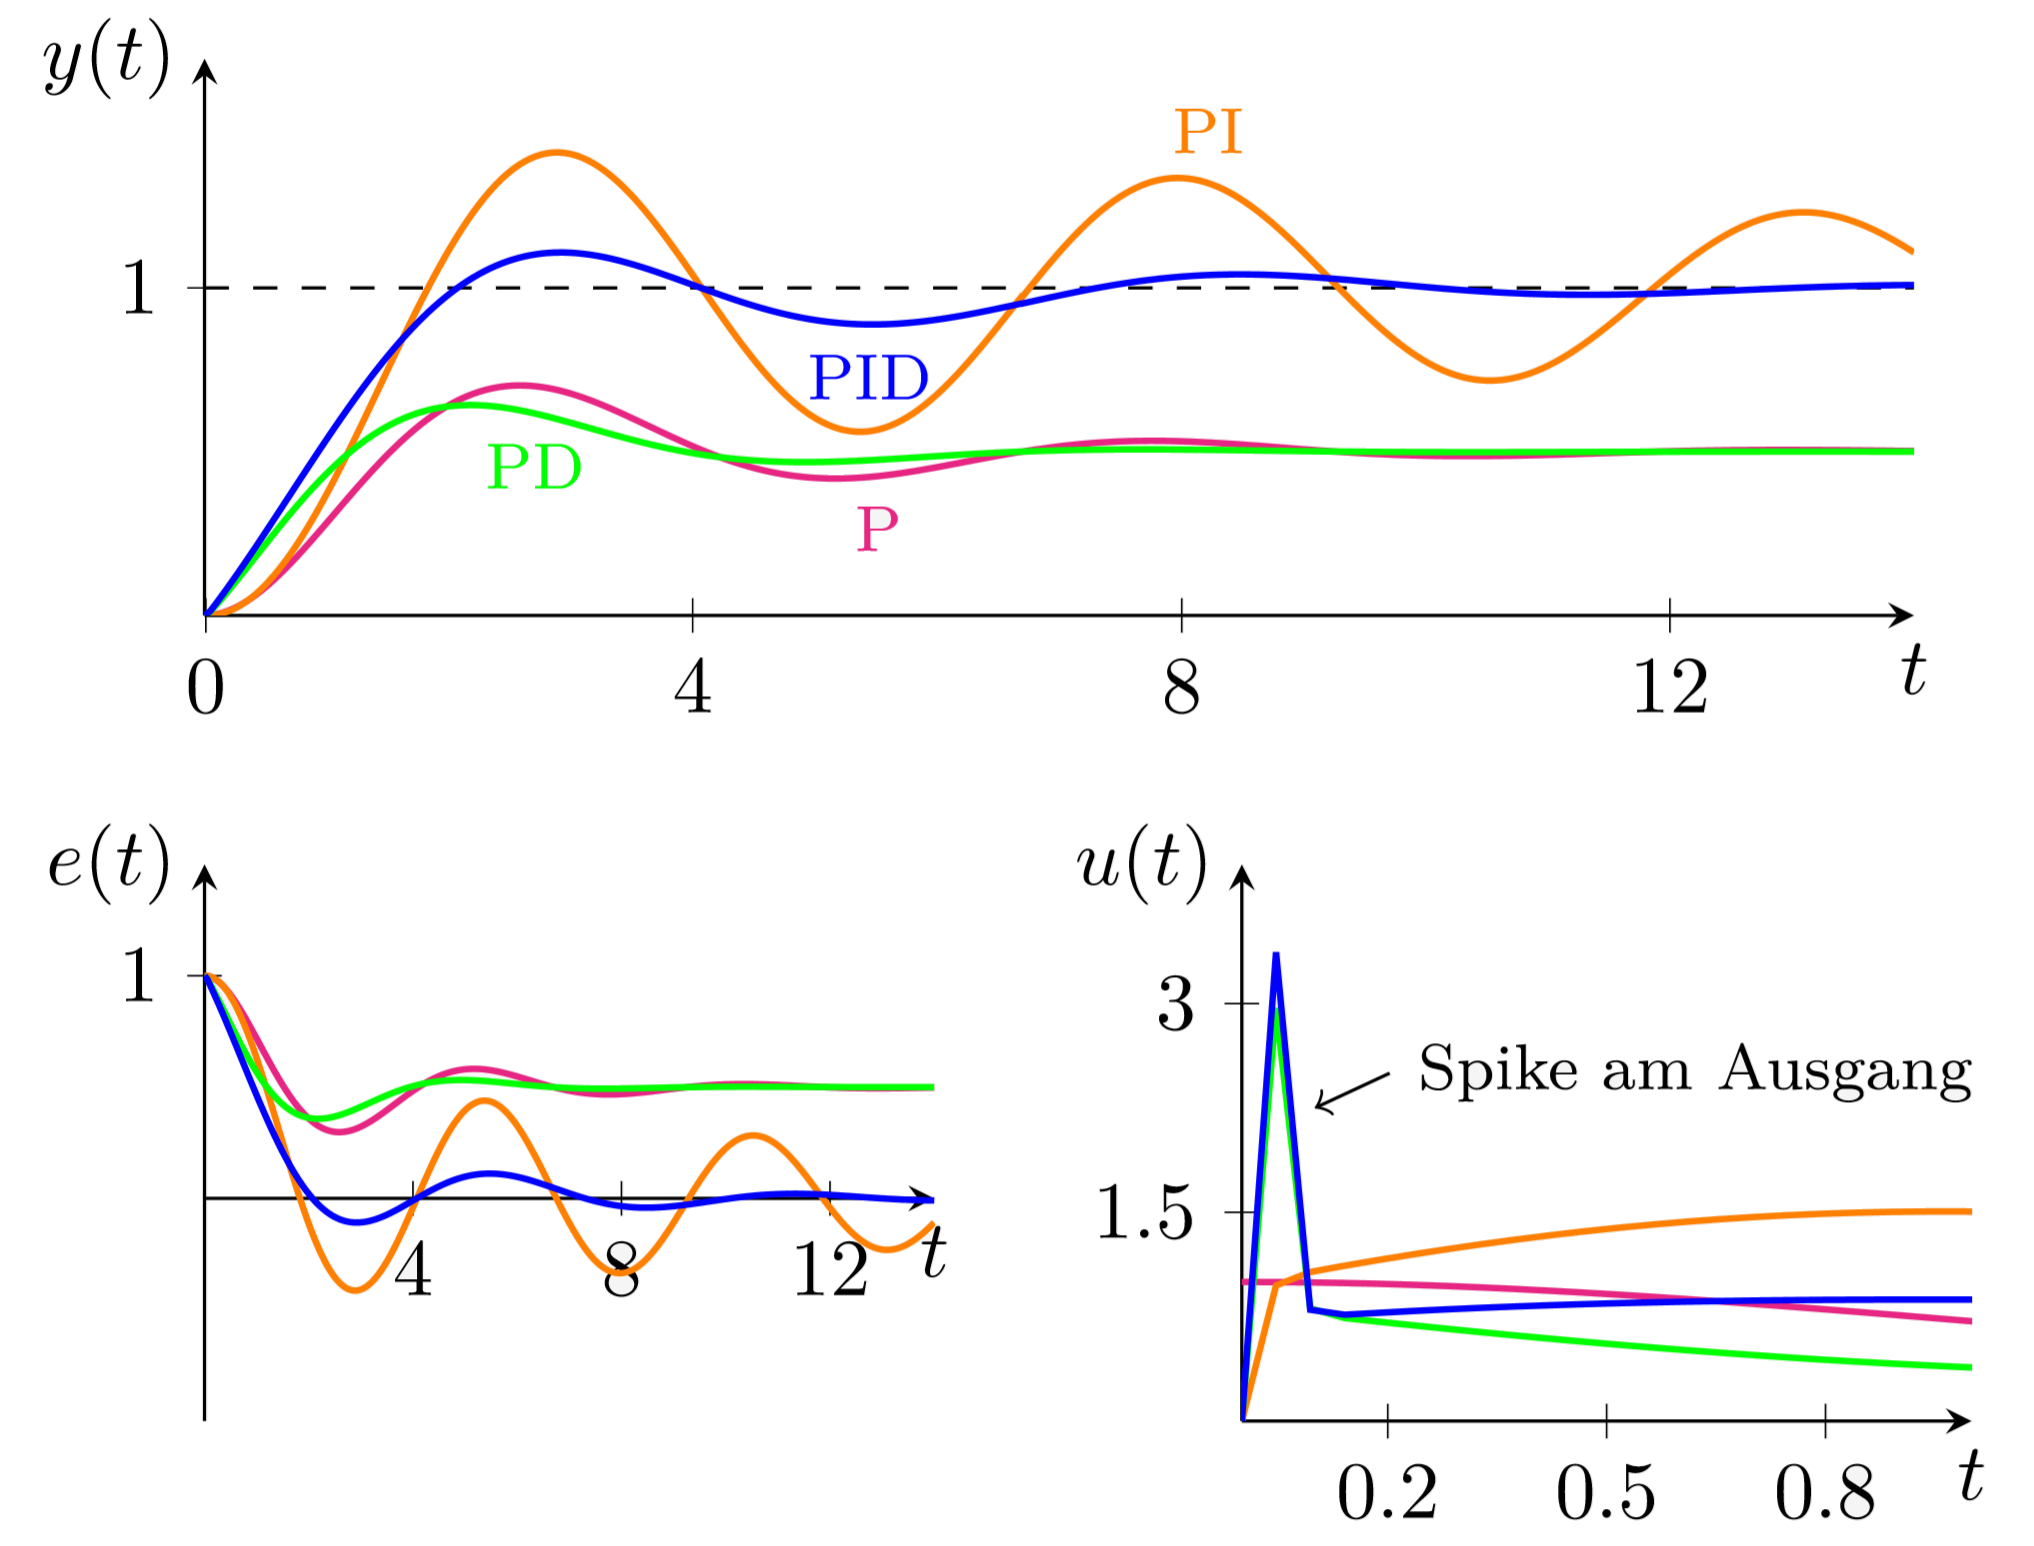
\includegraphics[width =\linewidth]{images/09/Bsp_PID.png}
            \end{center}
            Es ist ersichtlich, dass ein statischer Fehler durch den Integrator eliminiert werden kann. Der D-Term ermöglicht es, schneller auf die Fehleränderung zu reagieren, jedoch wird dadurch der Reglerausgang auch grösser.
\vfill\null\columnbreak            
        \subsubsection{Bsp}
            \textbf{Bode and Nyquist Plots of mass-oscillator example}
            \[P(s)=\frac{1}{(s+1)^2}\]
            \begin{center}
                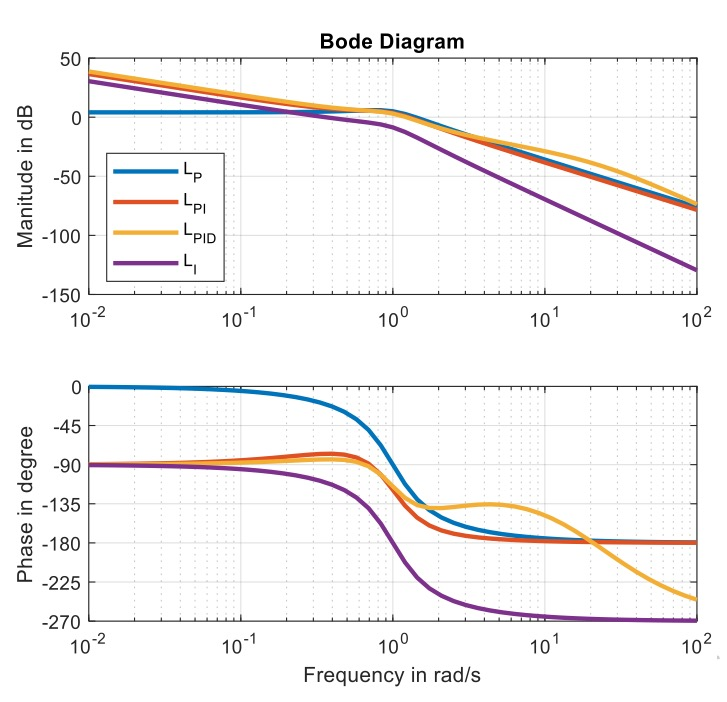
\includegraphics[width = 0.9\linewidth]{09/PID_Bode.jpg}
                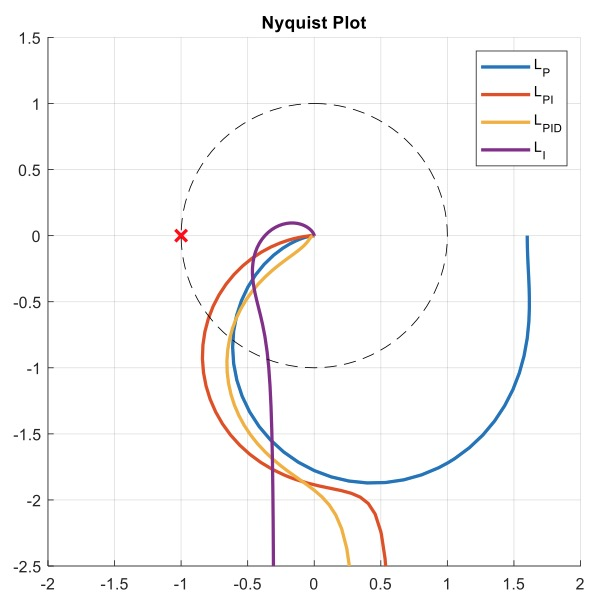
\includegraphics[width = 0.9\linewidth]{09/PID_Nyquist.jpg}
            \end{center}
    \subsection{PID-Regler Parameter Tuning nach Ziegler Nichols}
        Die Parameter $k_p,T_i$ und $T_d$ können durch extensives Testen des Systems bestimmt werden. Ein anderer Ansatz ist, der von Ziegler-Nichols. Hier geht man davon aus, dass das System $P(s)$ ein System erster Ordnung, mit zusätzlicher relativ kleiner Totzeit ist 
        \[P(s) \approx \frac{k}{\tau\cdot s + 1}\cdot e^{-T\cdot s},\hspace{3mm} \textrm{wobei:} \frac{T}{T+\tau}\overset{!}{<} 0.3\]
        Zur Bestimmung der Ziegler-Nichols Parameter startet man mit einem reinen P-Regler und erhöht die Verstärkung $k_p$ soweit, bis der geschlossene Regelkreis grenzstabil wird bei der Verstärkung $k_p^*$ (Pole von $T(s)$ auf der imaginären Achse). Falls die Modellannahme ungefähr stimmt, oszilliert das grenzstabile System bei $k_p^*$ mit einer Periode von $T^*$. Man kann diese Parameter des grenzstabilen System in folgende Tabellen einsetzen um Reglerparamter für verschiedene PID Kombinationen zu erhalten.
        \\$\omega^*$: Frequenz, bei der Phase $= -\pi$.
        \[\boxed{|k_p^* \cdot P(j\omega^*)| \overset{!}{=} 1} \hspace{3mm}
        \boxed{\angle k_p^* \cdot P(j\omega^*)\overset{!}{=}-\pi} \hspace{3mm}
        \boxed{T^* =\frac{2\pi}{\omega^*}}\]
        \begin{center}
        {\renewcommand{\arraystretch}{1.5}
            \begin{tabular}{l r r r}
            Regler & $k_p$ & $T_i$ & $T_d$ \\
                 \hline
                P & $0.5\cdot k_p^*$ & $\infty \cdot T^*$ & $0 \cdot T^*$ \\
                PI & $0.45\cdot k_p^*$ & $0.85\cdot T^*$ & $0 \cdot T^*$\\
                PD & $0.55 \cdot k_p^* $& $\infty \cdot T^*$ &  $0.15\cdot T^*$\\
                PID & $0.6\cdot k_p^*$ & $0.5 \cdot T^*$ & $0.125 \cdot T^*$\\
            \end{tabular}}
        \end{center}
    
        \subsubsection{Bsp}
            Gegeben sei folgendes System:  
            \[P(s) = \frac{1}{s(s+1)(s+2)}\]
            man soll mit Ziegler /Nichols ein Regler auslegen.
            Zur Bestimmung der kritischen Verstärkung $k_p^*$ und der kritischen Frequenz $\omega^*$ können die folgenden Beziehungen verwendet werden:
            \[k_p^* \cdot P(j\omega^*) \overset{!}{=} -1+0j\]
            Es folgt somit
            \begin{align*}
            \frac{k_p^*}{-j(\omega^*)^3-3(\omega^*)^2+2j\omega^*} &= -1\\
            k_p^* &= -(-3(\omega^*)^2 - j((\omega^*)^3-2\omega^*))\\
            k_p^* &= 3(\omega^*)^2+j((\omega^*)^3-2\omega^*)
            \end{align*}
            
            Aus dem Vergleich des Imaginärteils findet man 
            \[
            (\omega^*)^3-2\omega^* = \omega^* \cdot((\omega^*)^2-2) = 0\]
            Da wir nur an positiven realen Frequenzen ($k_p^* \in \mathbb{R}$) interessiert sind, folgt $\omega^*=\sqrt{2}$ Aus dem Vergleich der Realteilen folgt
            \[
            k_p^* = 3(\omega^*)^2 = 6
            \]
    \subsection{Iterative Loop Shaping}
        Ein System, das mit einem PID-Regler ausgelegt wird, erfüllt unter Umständen nicht alle Designspezifikationen. Um gewisse Frequenzbänder nach Wunsch abzuändern, kann man einen beliebigen Regler zum Beispiel mit Lead-/Lag- Elemente erweitern oder einen Regler von Grund auf neu
        erstellen. 
    \subsection{Lead-Lag Elemente 1. Ordnung}
        der Term 'Lead-Lag' bezeichnet zwei Arten von Systemen mit gleicher Struktur und den zwei Parametern $\alpha$ und $T$:
        \[
        C(s) = \frac{T\cdot s + 1}{\alpha \cdot T \cdot s + 1}, \hspace{3mm} \alpha,T\in \mathbb{R}_+
        \]
        Der Wert von $\alpha$ definiert ob es sich um ein Lead- oder ein Lag- Element handelt: 
        \begin{align*}
            0 &< \alpha < 1 & \Leftrightarrow \textrm{Lead-Element} \\
            1 &< \alpha     & \Leftrightarrow \textrm{Lag- Element}
        \end{align*}
        Die Parameter $\alpha$ und $T$ werden gezielt gewählt, sodass bei der Frequenz $\hat{\omega}$ eine maximale Phasenänderung von $\hat{\varphi}$ vorliegt:
        \[\alpha = \Big(\sqrt{\tan^2(\hat{\varphi}+1}-\tan(\hat{\varphi})\Big)^2, \hspace{3mm} T = \frac{1}{\hat{\omega}\cdot\sqrt{\alpha }}\]
        \begin{center}
            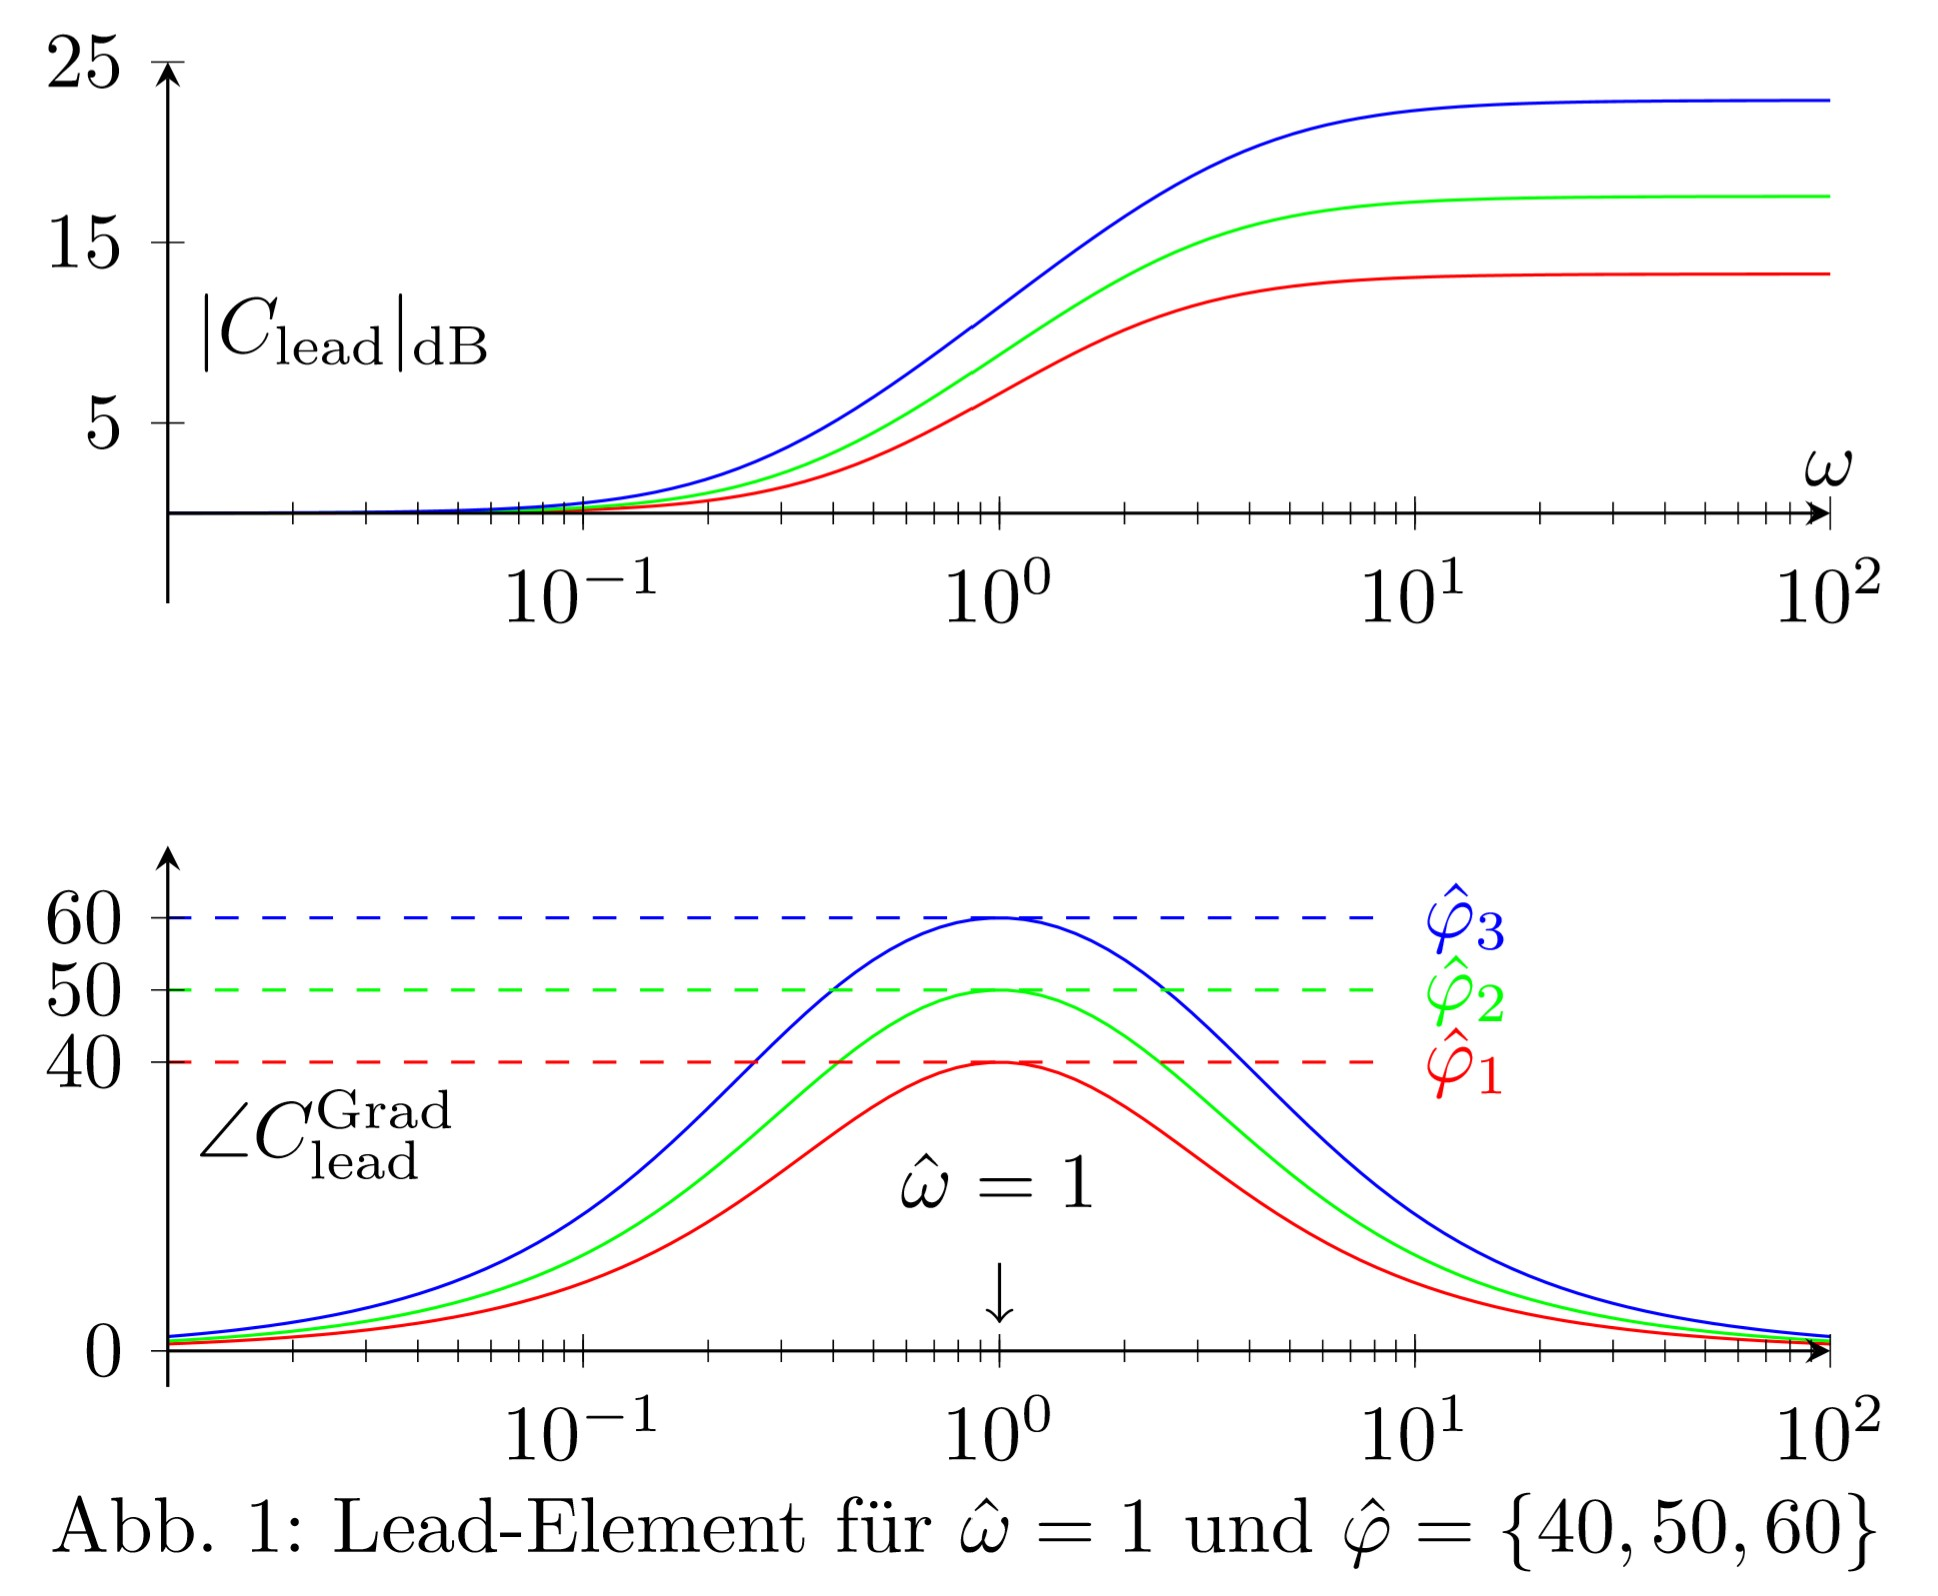
\includegraphics[width = 0.85\linewidth]{images/09/Lead_Lag_pos.jpg}
            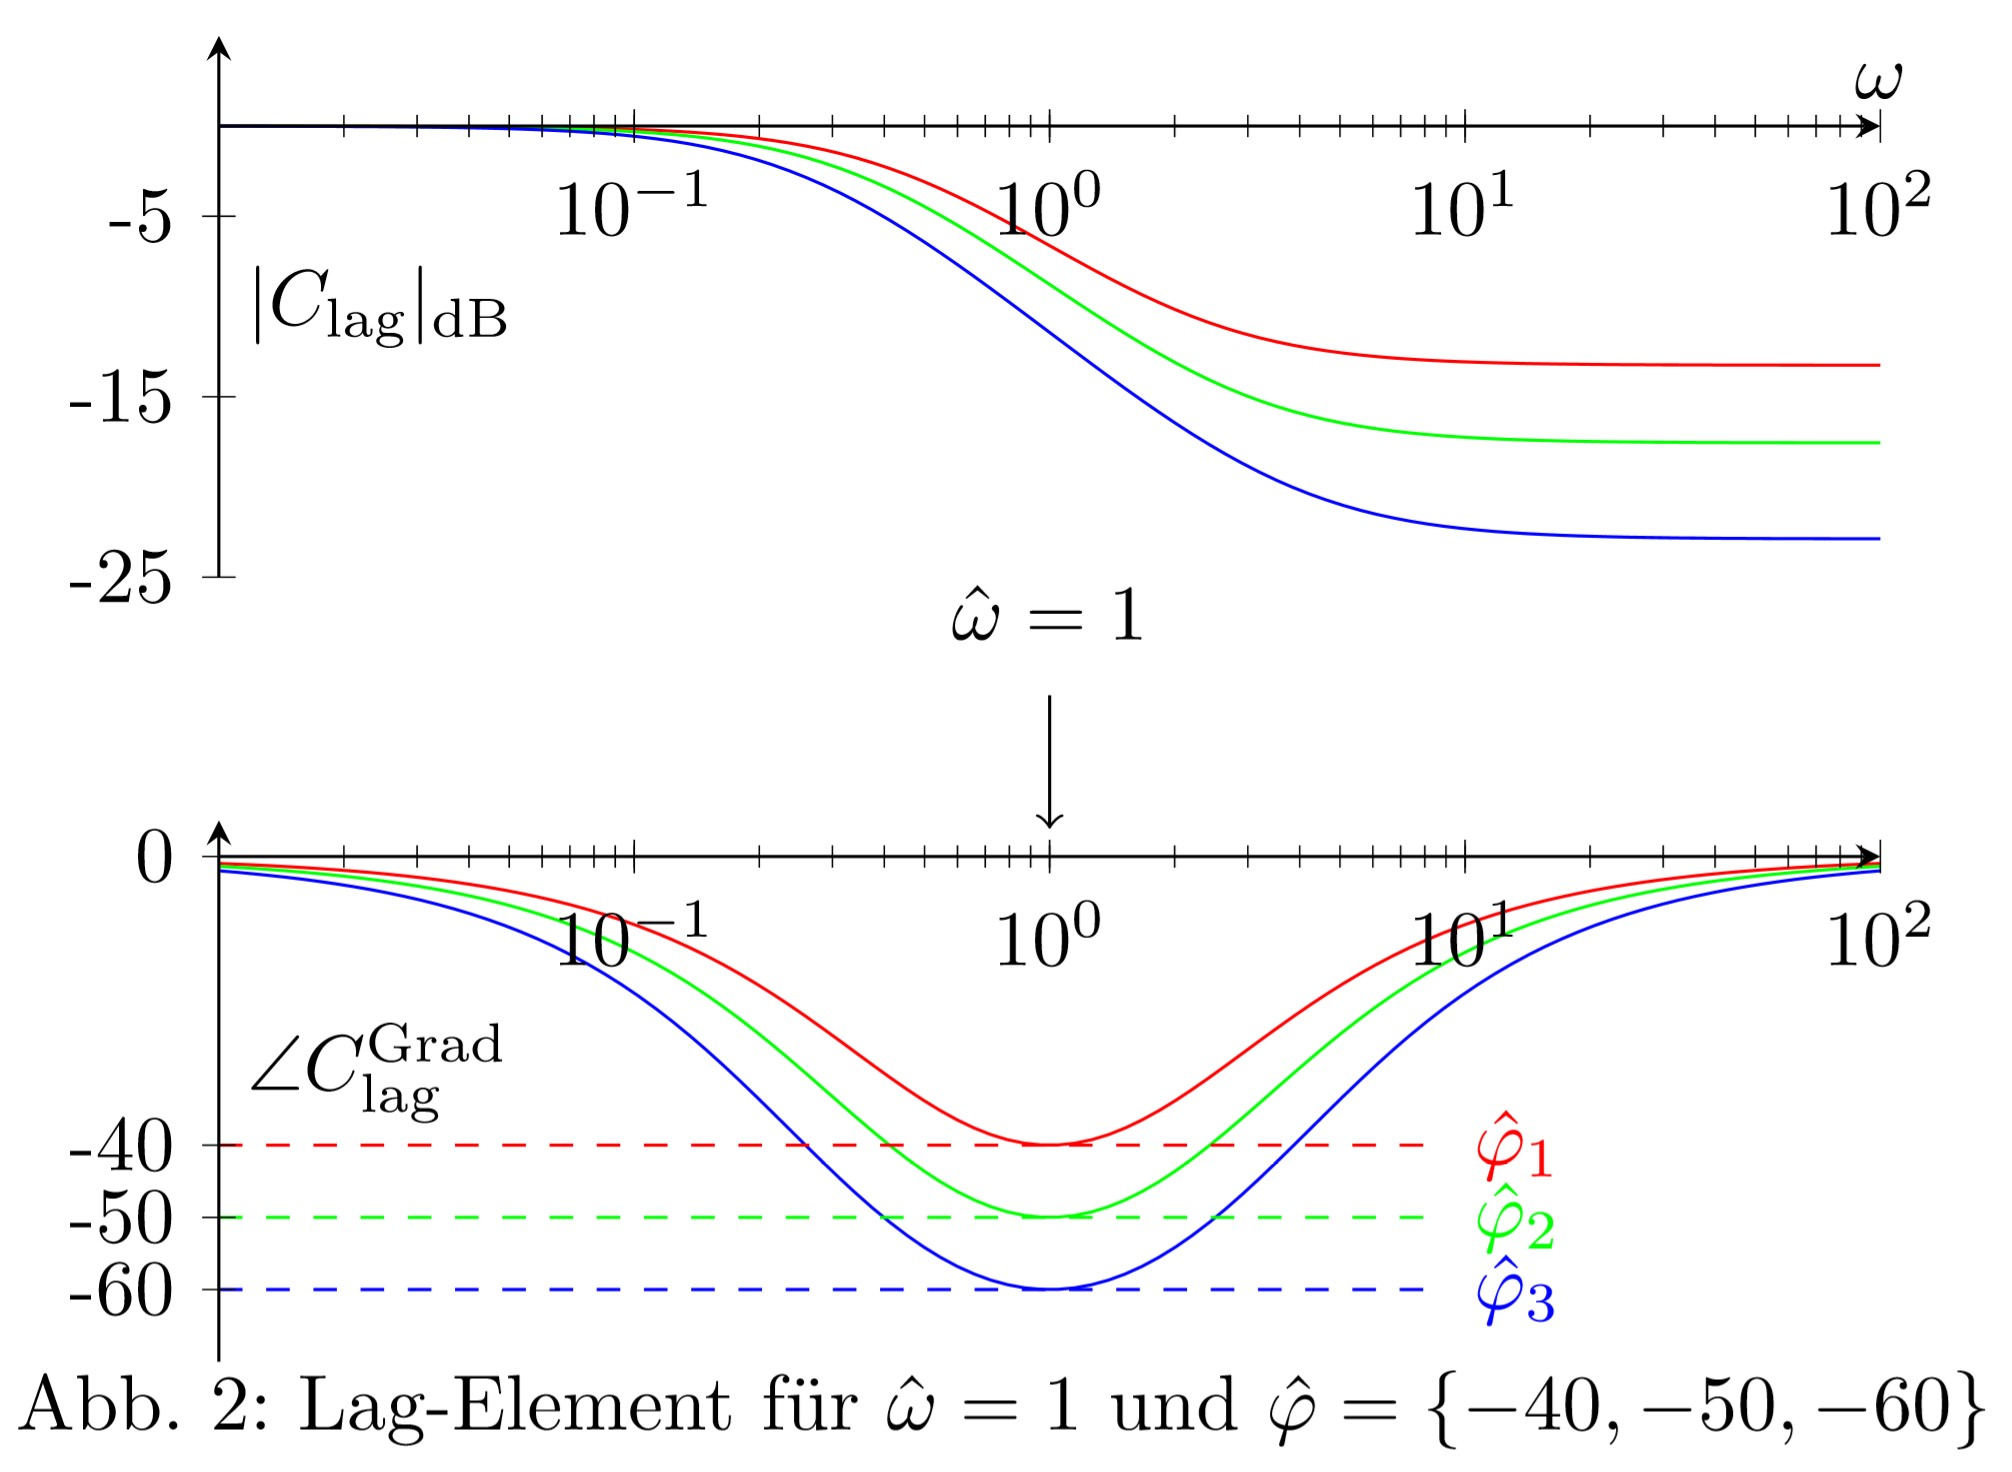
\includegraphics[width = 0.8\linewidth]{images/09/Lead_Lag_neg.jpg}
        \end{center}
        Ein Lag- Element mit $-\hat{\varphi}$ entspricht einer Spiegelung des Magnituden und Phasendiagramms des Lead-Elements mit $\hat{\varphi}$.
    \subsection{Lead-Lag Elemente 2. Ordnung}
        Die Verwendung eines Elements 1. Ordnung beeinflusst Frequenzen in der grösseren Umgebung von $\hat{\omega}$. Die Idee eines Elements 2. Ordnung ist, dass der gewünschte Effekt an einer bestimmten Frequenz besser isoliert ist. Die Struktur erfordert die Parameter $\kappa, \epsilon,$ und $\omega_0$
        \[
        C(s) = k\cdot\frac{s^2 +2\cdot\kappa\cdot\epsilon\cdot(1-\epsilon)\cdot\omega_0\cdot s+(1-\epsilon)^2\cdot\omega_0^2}{s^2+2\cdot\kappa\cdot\epsilon\cdot(1+\epsilon)\cdot\omega_0\cdot s+(1+\epsilon)^2\cdot\omega_0^2}\]
        
        Zusätzlich zur Wahl der mittleren Frequenz $\hat{\omega}$ und der maximalen Phasenverschiebung $\hat{\varphi}$ kann man nun zusätzlich die Breite des Frequenzbands durch den Parameter $\epsilon$ wählen:
        \[ k = \frac{(1+\epsilon)^2}{(1-\epsilon)^2},\hspace{3mm} \kappa=\frac{\cot(\hat{\varphi}/2)}{\sqrt{1-\epsilon^2}},\hspace{3mm} \omega_0 = \frac{\hat{\omega}}{\sqrt{1-\epsilon^2}}\]
        \begin{center}
            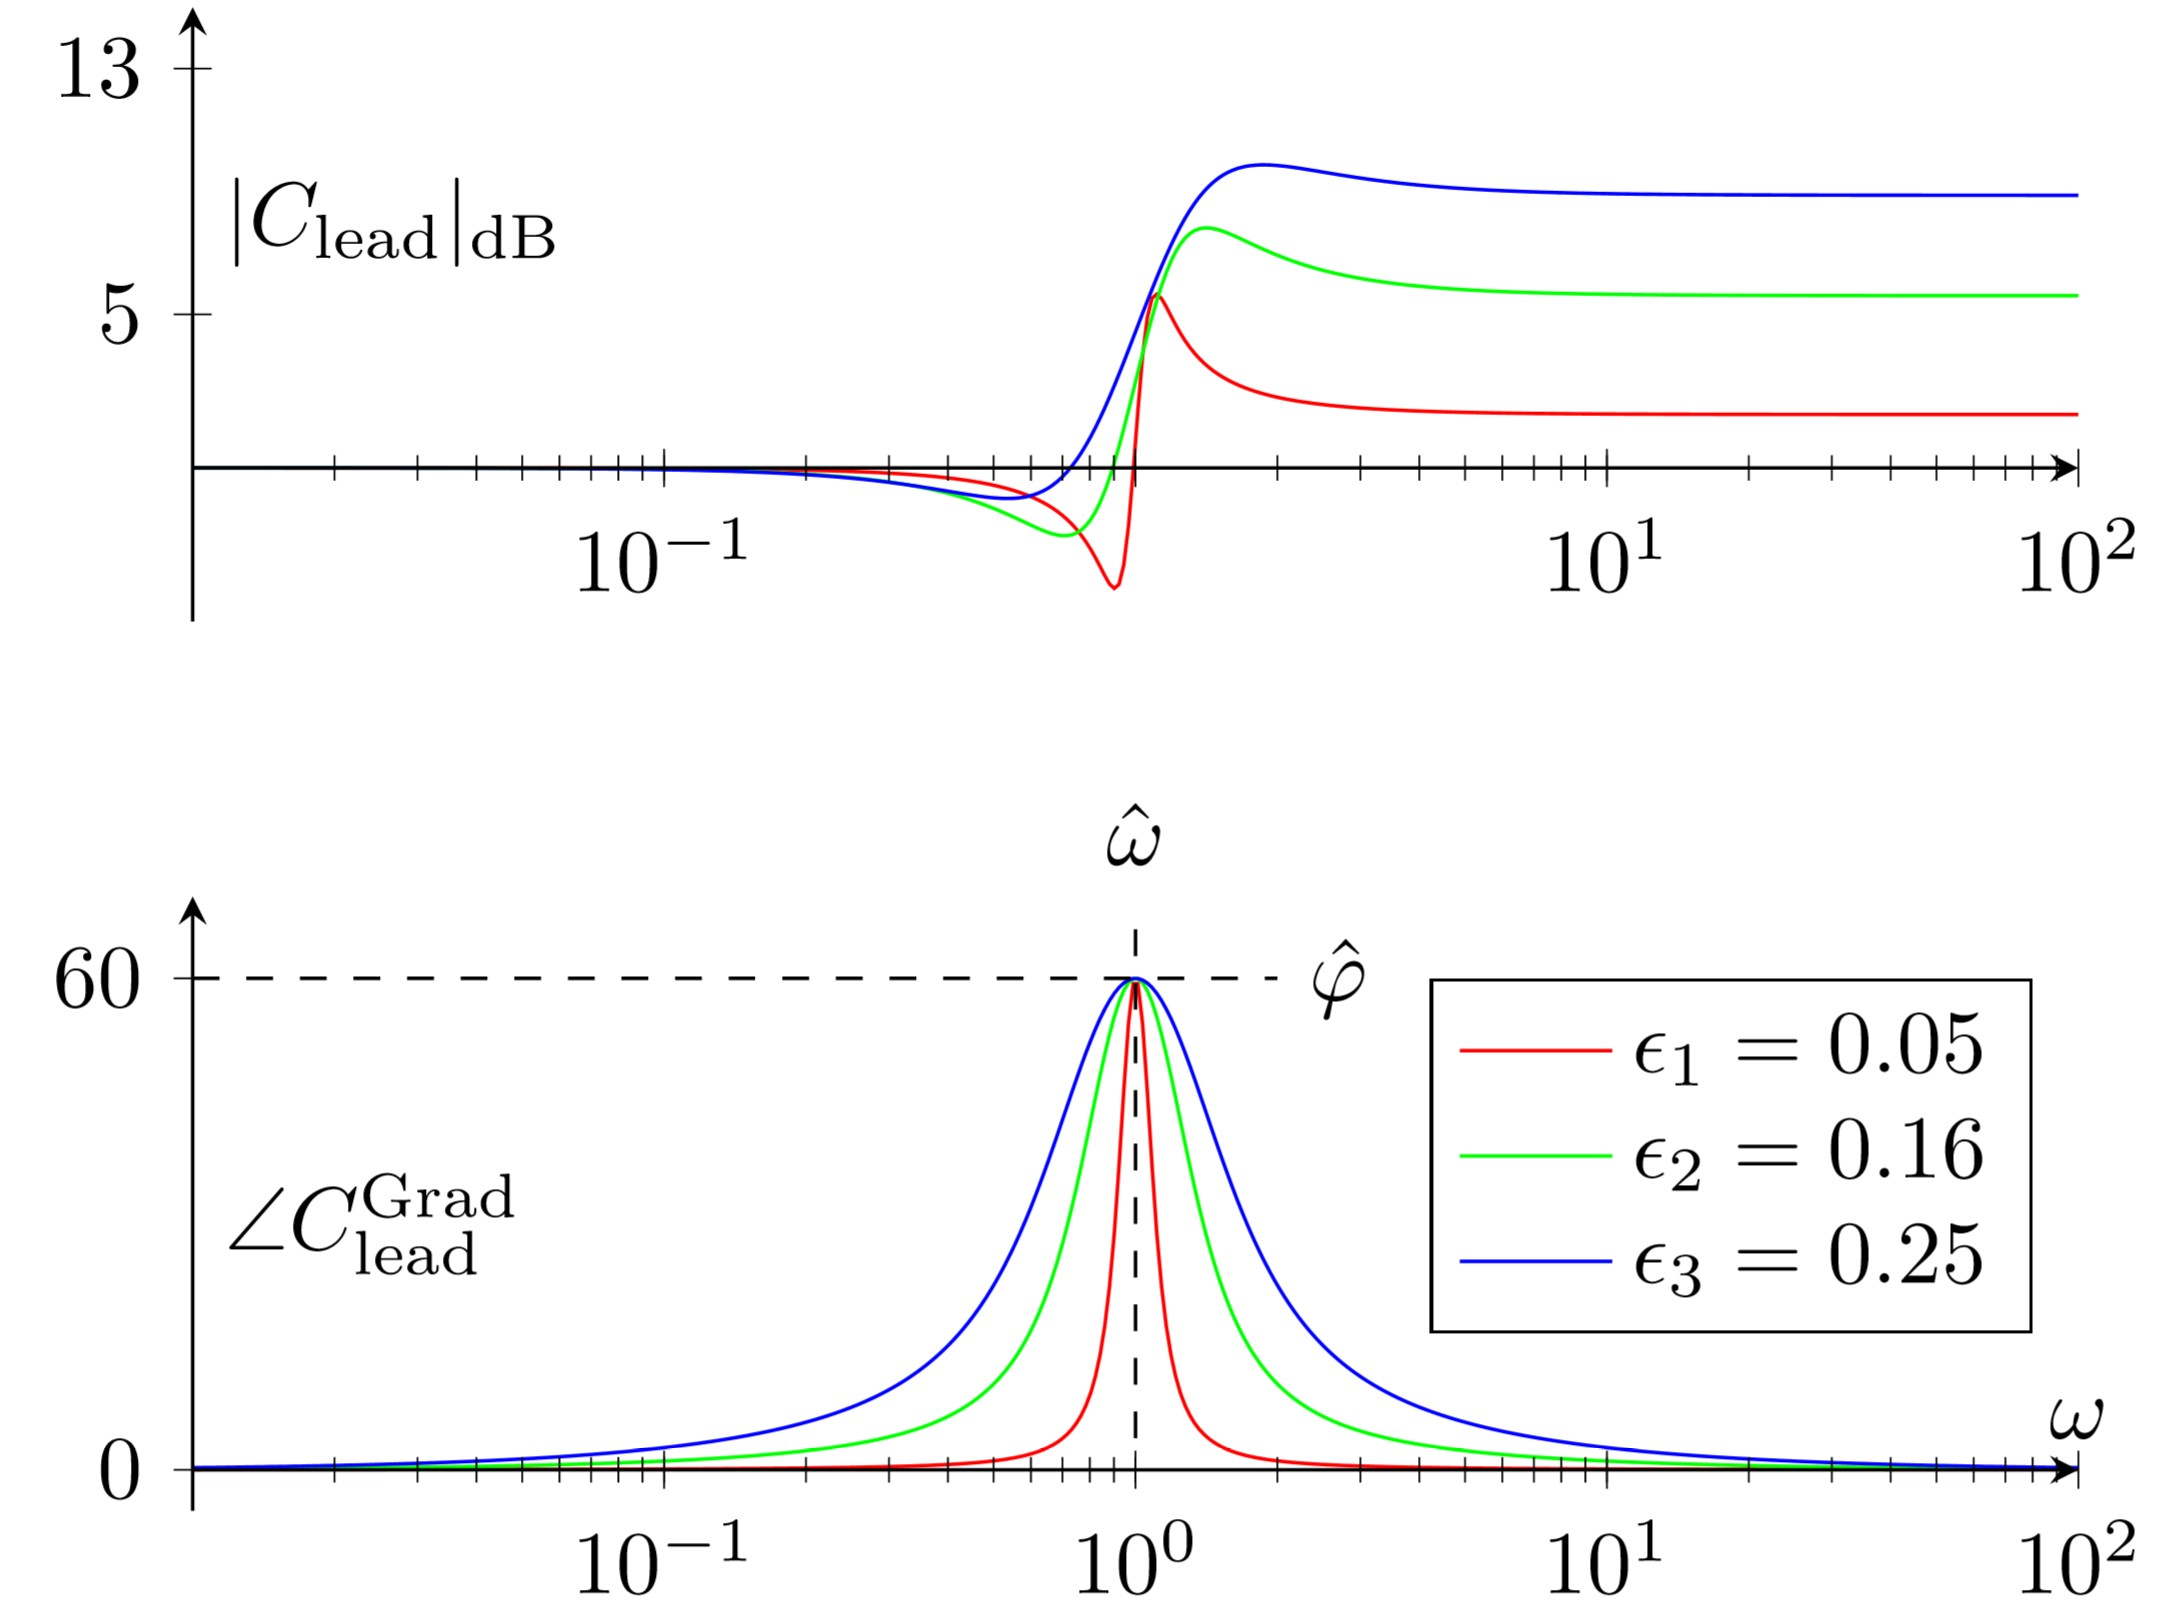
\includegraphics[width = 0.8\linewidth]{images/09/Lead_Lag_2.jpg}
        \end{center}
            
    \subsection{Inversion der Regelstrecke}
        Wenn die Regelstrecke $P(s) = \frac{n_p(s)}{d_p(s)}$ mit relativem Grad $r$ asymptotisch stabil ist und nur minimalphasige Nullstellen enthält, kann ein Regler $C(s)$gewählt werden, der die Dynamik der Regelstrecke exakt kompensiert und gleichzeitig in einer gewünschten Übertragungsfunktion $L(s)$ des offenen Regelkreises resultiert:
        \begin{align*}
            L(s) &= P(s)\cdot \underbrace{P(s)^{-1}\cdot\overbrace{\frac{1}{T_i\cdot s}\cdot\frac{1}{(\tau\cdot s + 1)^{r-1}}}}^{\textrm{desired }L(s)}_{C(s)}\\
            \Rightarrow C(s) &= P(s)^{-1}\cdot\frac{1}{T_i\cdot s}\cdot\frac{1}{(\tau\cdot s + 1)^{r-1}}\\
            C(s) &= \frac{d_p(s)}{n_p(s)}\cdot\frac{1}{T_i\cdot s}\cdot\frac{1}{(\tau\cdot s + 1)^{r-1}}
            \end{align*}
            
        Der Regler invertiert die Dynamik der Regelstrecke, und somit haben die Pole und Nullstellen von $P(s)$ keinen Einfluss auf die Übertragungsfunktion des offenen Regelkreises $L(s$. Die übrigen Elemente von C(s) stellen sicher, dass die gewünschte Übertragungsfunktion $L(s)$ des offenen Regelkreises resultiert:
        \[L(s) = \frac{1}{T_i\cdot s}\cdot \frac{1}{(\tau\cdot s + 1)^{r-1}}\]
        Mit der Verstärkung $T_i = \omega_c^{-1}$ kann die gewünschte Durchtrittsfrequenz $\omega_c$ eingestellt werden. Zusätzlich wählen wir $\tau < T_i$ und $\omega_c < \omega_2$.
        
    \subsection{Bsp maximale Totzeit}
        Für welche maximale Totzeit $e^{-\tau s}$ ist der geschlossene Regelkreis (mit $C(s)=k_p=1$ noch stabil?
        \begin{enumerate}
            \item $\omega_c$ bei dem $|\Sigma(S)|=0 dB$ aus Bode auslesen.
            \item Phasenreserve $\varphi$ in radian berechnen
            \item $\tau_{max}=\frac{\varphi}{\omega_c}$
        \end{enumerate}